\usepackage{hyperref}
\startreport{The Tesla ``Sum of Squares'' Bug}
\reportauthor{Ramesh Subramonian}

\section{Introduction}

Recently, an error was discovered in the way statistics were being
computed in Tesla. To quote, ``This find impacts the Rubix BE
deliverables profoundly.''

The Q implementation of the Tesla back-end suffered from the same bug.
In this document, we describe how the bug was fixed using Q.
I would like to draw the reader's attention to:
\be
\item The simplicity of the solution --- it is no more than a few lines
of code
\item The efficiency of the solution --- the run times are within reason
\ee

The conclusion is that {\bf agility } is a key requirement of any analytics
solution we put together. 
This is not the first time nor the last time that changes will need 
to be made to the way we transform data. 
We will need to respond to the business in
days, not weeks. 

Even in this case, 
\bi
\item we thought we had fixed the bug
(Section~\ref{The_Fix}). 
\item then we found that there wasn't an
agreement on what the fix should be (Section~\ref{The_Debate}). 
\item this  required us to implement
another solution (Section~\ref{The_Next_Fix}).
\ei

I find myself these days preaching about the lessons engineers can learn
from the humanities. Here is a quote which illustrates the point
\footnote{Three Men in a Boat by Jerome K. Jerome}.

{\it 
Let your boat of life be light, packed with only what you need \ldots 
You will find the boat easier to pull then, and it will not be so
liable to upset, and it will not matter so much if it does upset;
good, plain merchandise will stand water. You will have time to think
as well as to work.
}

\section{The Bug}
\label{The_Bug}

Quoting Omar, ``we found a bug in the cross-day aggregation logic where 
the total square is being calculated incorrectly.'' Details in
\url{https://iwww.corp.linkedin.com/wiki/cf/x/_zGwB}

Further, ``The
change required to implement the new logic is large because the cubes
and queries were optimized based on the ``current computation'' logic. The
correct computation would require that we maintain the member level
information (associated with the metric) and this results in a massive
increase in space and computation.''

\section{The Spec}

The ``correct'' specification is in Figure~\ref{tesla_spec}, borrowed
from
\url{https://iwww.corp.linkedin.com/wiki/cf/x/_zGwB}


\begin{figure}
\centering
\fbox{
  \begin{minipage}{12 cm}
  \centering
  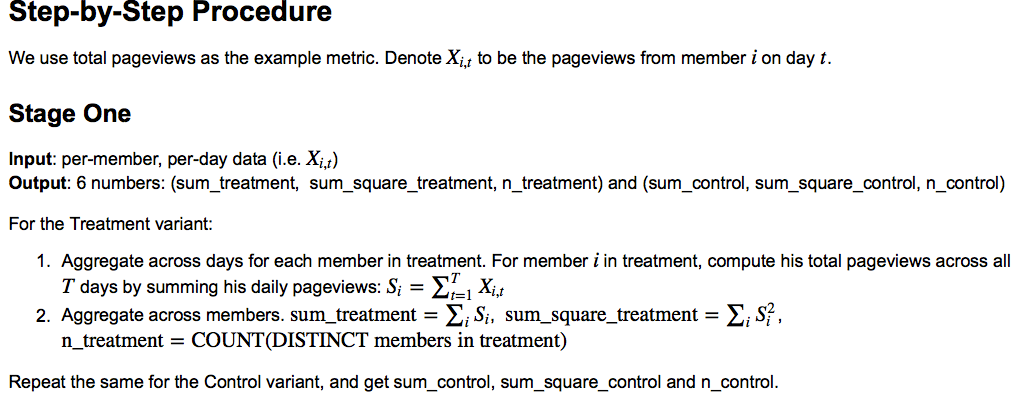
\includegraphics[width=4.5in]{tesla_spec.png}
  \caption{Tesla Spec}
  \label{tesla_spec}
  \end{minipage}
}
\end{figure}

\section{The Data Model}
\label{The_Data_Model}
Recall that Q is a column-store database. The data model we use 
\be
\item stores each day's data in a separate table
\item for a given date, 
\be
\item each row corresponds to a member who visited the site that day
\item we have one column for each metric (some cells may be null)
\item we have one column for each experiment that was alive that day, 
the values being the different treatments (some cells may be null). 
The values may also be a
combination of treatment and segment. In either case, we do not
anticipate more than 256 different values for a given experiment column.
\ee
\ee
Let us do some back-of-the-envelope calculations to assess the storage
needs of this data model. Assume 
\be
\item 32M members per day, \(2^{25}\)
\item 512 metrics \(2^9\)
\item 4096 experiments, \(2^{12}\)
\item a metric can be stored in an average of 1 byte (some will be 2
    bytes, some will be 1 bit)
\item an experiment can be stored in 1 byte 
\item assume 32 days in a month, \(2^5\)
\ee
This means that a month's data is 
\(2^5 \times 2^{25} \times (2^2 + 2^9 + 2^{12}) \approx \) 4 TB.
We do not believe that this is excessive
\section{The Fix}
\label{The_Fix}

As Omar indicates, we need to accumulate the values of the metric for
{\bf each} member, over the desired time period, {\bf before} squaring it. The
following code does the job.  In this example, 
\bi
\item We used {\it number of page views} as the metric. m75 is our internal
  name for it. 
\item We used {\it search-voltron-use} as our experment.
\verb+fk_lkp_treatment_1+ is our internal name for it.
\item We used the first 7 days of May as our test period
\item It takes approximately one second to process one metric over one
day.  
\item Current implementation stores the metric as 4-bytes. Given
that it is unlikely that a real member would visit more than 32767
pages in a day, this could be stored in 2 bytes. Given that memory
access is the dominant cost, this simple compression could cut the
time in half.
\item We believe that 0.5 seconds/metric/day is within striking
distance. Sathya describes a typical calculation s consisting of 50 
metrics over the last 14 days. This would take 10 minutes on one
machine.
\ei
\begin{verbatim}
date=20130501
mfld=m75
tkfld=fk_lkp_treatment_1
# TM contains member IDs of all members in last 30 days
while [ $date -le 20130507 ]; do
  mtbl=TM$date # contains information about that date
  if [ $iter = 1 ]; then
    q srt_join $mtbl mid $mfld TM mid sum_vals reg
  else
    q srt_join $mtbl mid $mfld TM mid temp_fld reg
    q f1f2opf3 TM temp_fld sum_vals '+' sum_vals
  fi
  date=`expr $date + 1` # use better way to find next date
done
q f1f2opf3 TM sum_vals sum_vals '*' sqr_sum_vals
q delete   TM temp_fld
q countf   TM sum_vals     $tkfld '' lkp_treatment sum_vals
q countf   TM sqr_sum_vals $tkfld '' lkp_treatment sqr_sum_vals
\end{verbatim}

\section{The Debate}
\label{The_Debate}

However, the above solution glosses over the fact that a member could
change treatment during the lifetime of an experiment. There does not
appear to be consensus as to whether it is okay to ignore this. So, the
solution in the next section deals with what happens when we need to
aggregate by member and treatment (not just by member) before the
squaring is done. 

\section{The Next Fix}
\label{The_Next_Fix}

There was no significant change in run time for the following approach
--- about 1 second per metric per day without optimization.

\begin{verbatim}
date=20130501
mfld=m75
tkfld=fk_lkp_treatment_1
q delete Tcomp:tempt
mask=16777215 # masks all but lowest 24 bits
while [ $date -le 20130507 ]; do
  mtbl=TM$date
  # compfld = (mid << 32) | (treatment << 24) | metric
  # This means 32 bits for mid, 8 for treatment, 24 for metric
  q pack $mtbl mid:$tkfld:$mfld 32:24:0 I8 compfld
  q set_meta $mtbl compfld sort_type ascending # Dangerous but correct
  if [ $iter = 1 ]; then
    q copy_fld $mtbl compfld '' Tcomp
  else
    q t1f1t2f2opt3f3 $mtbl compfld Tcomp compfld pvalcalc "mask=[$mask]" tempt compfld
    q rename tempt Tcomp 
  fi
  q set_meta Tcomp compfld sort_type ascending # Dangerous but correct
  date=`expr $date + 1`
done
q f1s1opf2 Tcomp compfld    $mask      '&' sum_metric
q f1f2opf3 Tcomp sum_metric sum_metric '*' sqr_sum_metric
q f1s1opf2 Tcomp compfld    24 '>>' $tkfld
q f1s1opf2 Tcomp $tkfld     255 '&' $tkfld

q countf   Tcomp sum_metric     $tkfld '' lkp_treatment sum_vals
q countf   Tcomp sqr_sum_metric $tkfld '' lkp_treatment sqr_sum_vals
\end{verbatim}
